% =====================================================================
% Paper Tecniacústica 2026 — versión de envío en doble ciego.
%
% Compilar con:  pdflatex paper.tex
% (dos pasadas para resolver referencias internas)
% =====================================================================
\documentclass{tecniacustica}

\title{¿Cómo suena una gota que rueda? Un marco paramétrico físicamente informado para la síntesis de sonidos imposibles}

\begin{document}
\maketitle

\pacs{43.60.Lq, 43.58.Ta, 43.60.Uv}

\authorsblock{%
  \textit{[Doble ciego: autores y afiliaciones se añaden tras revisión]}
}

\keywords{síntesis de sonido, Foley, física-DSP, sonidos imposibles, DDSP, inversión de parámetros}

\vspace{0.5em}

\begin{resumen}
El diseño sonoro audiovisual requiere con frecuencia combinaciones materia--interacción que no ocurren en la naturaleza: una gota líquida que rueda, un impacto rocoso húmedo, grava raspando bajo agua. Los enfoques generativos basados en codificadores neuronales preentrenados permiten manipular el espacio latente y producen variación medible en métricas espectrales, pero raramente se traducen en cambios que el oyente identifique semánticamente como ``más líquido'' o ``más rocoso''. Este trabajo propone un marco paramétrico físicamente informado organizado en capas modulares — síntesis modal, fricción de cuerpo y superficie, granular estocástico, eventos de gota con dinámica de Minnaert — combinadas por un compositor genérico que admite especificaciones de material, interacción y modificadores. Cada parámetro tiene significado físico directo, garantizando que un control ``más X'' corresponda a una transformación acústica coherente. Como caso paradigmático presentamos la gota rodante, sin referente natural directo. Sobre 75 mediciones (15 pares escena--parámetro por cinco métricas acústicas), 10 de 15 pares producen variación monotónica significativa ($|\rho_\mathrm{Spearman}| > 0,7$); de los cinco restantes, cuatro corresponden a parámetros sin efecto en su escena. Una contraparte diferenciable del motor permite recuperar parámetros físicos por descenso de gradiente desde grabaciones, con errores del orden del 1\,\% o inferiores en gotas e impactos modales. Discutimos el posicionamiento del marco frente al estado del arte reciente en acústica de burbujas acopladas y en modelado físico diferenciable, e identificamos el principal cuello de botella de la inversión — la estimación de frecuencia por descenso de gradiente sobre pérdidas espectrales — como una patología intrínseca que sitúa a la gota rodante en el extremo mal condicionado de un continuo de identificabilidad. Extendemos además el marco con un mecanismo de fusión de identidad entre materiales dispares — quimeras auditivas con alineación de registro físicamente exacta vía la relación de Minnaert — y mostramos que un índice compuesto para ordenar los candidatos resultantes queda anticorrelado con el defecto perceptual que pretende detectar ($r=+0,42$ con el factor de cresta): un resultado negativo que documentamos sin atenuar y que repite, en la fusión, la misma disociación entre monotonía cuantitativa y perceptual que estructura el resto del artículo.
\end{resumen}

\begin{englishabstract}
Audiovisual sound design routinely requires material--interaction combinations that do not occur in nature: a rolling liquid droplet, a wet rock impact, gravel scraping under water. Generative approaches based on pretrained neural codecs allow latent-space manipulation and yield measurable variation in spectral metrics, but seldom translate into changes that listeners semantically identify as ``more liquid'' or ``more rocky''. We propose a physics-informed parametric framework organised in modular layers --- modal resonators, body-and-surface friction, stochastic granular events, droplet events with Minnaert bubble dynamics --- combined by a generic composer that accepts material, interaction and modifier specifications. Each parameter has direct physical meaning, so that a ``more X'' control produces an acoustically coherent transformation. As paradigmatic case we present the \emph{rolling droplet}, which has no direct natural referent. Across 75 measurements (15 scene--parameter pairs over five acoustic metrics), 10 of 15 pairs produce significant monotonic variation ($|\rho_\mathrm{Spearman}| > 0.7$); of the remaining five, four correspond to parameters with no effect on their scene. A differentiable counterpart of the engine recovers physical parameters by gradient descent from recordings, with errors at or below the 1\,\% range on droplet and modal impact events. We position the framework against recent state of the art in coupled-bubble acoustics and differentiable physical modelling, and identify the main bottleneck of the inverse problem --- frequency estimation by gradient descent on spectral losses --- as an intrinsic pathology that places the rolling droplet at the ill-conditioned end of an identifiability continuum. We further extend the framework with an identity-fusion mechanism across disparate materials --- auditory chimeras with physically exact register alignment via the Minnaert relation --- and show that a composite index for automatically ranking the resulting candidates is anticorrelated with the perceptual defect it is meant to detect ($r=+0.42$ with crest factor): a negative result we report without softening, which repeats, in fusion, the same dissociation between quantitative and perceptual monotony that structures the rest of the paper.
\end{englishabstract}

% ============================================================
\section{Introducción}
% ============================================================

El diseño sonoro para cine, animación, videojuegos y medios inmersivos requiere a menudo sonidos que \emph{no} existen como grabaciones. Una animación pide una gota de mercurio que rueda; un equipo de audio para videojuegos necesita grava raspando dentro de una cueva inundada; una pieza experimental busca una roca líquida. Dos rutas han dominado la práctica.

La primera, el \textbf{Foley clásico}, combina capas grabadas en estudio que se procesan manualmente. El resultado es de gran calidad pero costoso, lento y poco reproducible: no existe una forma sistemática de pedir ``más mojado'' o ``menos granuloso'' sobre un evento existente.

La segunda, los \textbf{enfoques generativos neurales} basados en codificadores preentrenados (EnCodec~\cite{defossez2022encodec}, RAVE~\cite{caillon2021rave}, DAC~\cite{kumar2023dac}) o difusión latente condicionada por texto (AudioLDM~\cite{liu2023audioldm}, Stable Audio Open~\cite{evans2024stableaudio}), promete una ruta más rápida. Pero presenta dos limitaciones recurrentes. Primero, los espacios latentes de los codificadores preentrenados están optimizados para \emph{reconstrucción general de audio}, no para representar semántica de material o interacción, y sus ejes carecen de anclaje en atributos físicos. Segundo, cuando se manipulan estas representaciones para obtener mezclas tipo ``más líquido'' o ``más rocoso'', el espectro cambia de forma medible (RMS, rango dinámico, centroide), pero el carácter percibido del sonido a menudo \emph{no} cambia: el oyente no oye un líquido donde no lo había~\cite{roche2021autoencoders,devis2023control}.

Esta disociación entre \emph{monotonía cuantitativa} en el espacio de métricas y \emph{monotonía perceptual} en el espacio del audio es un obstáculo central para el control interpretable. Proponemos atacar el problema desde el extremo opuesto: en lugar de partir de un espacio latente aprendido y esperar que codifique significado físico, construimos un motor de síntesis paramétrico cuyos controles \emph{son} parámetros físicos por construcción. Bancos de resonadores modales reproducen cuerpos materiales; modelos de fricción reproducen raspados y arrastres; trenes granulares estocásticos reproducen grava y arenas; la resonancia de Minnaert reproduce la formación de burbujas de aire en agua. Un compositor genérico combina estas primitivas a partir de una especificación de material, interacción y modificadores de alto nivel, y expone controles físicos continuos — humedad, granularidad, rigidez, resonancia, continuidad — que el usuario manipula como deslizadores.

El resultado es un marco donde más humedad incrementa la viscosidad de la gota, más granularidad aumenta la rugosidad de la trayectoria de rodadura, y más rigidez desplaza las fundamentales modales hacia arriba: cada control produce una transformación audible coherente con su significado físico. El caso de la \textbf{gota rodante} — un sonido sin referente natural que podamos grabar — ilustra el enfoque como un tren cuasi-periódico de contactos modulados por velocidad y rugosidad sobre una sutil cola modal de la superficie.

Las contribuciones de este trabajo son: (i) una biblioteca modular de primitivas físicamente informadas para efectos de sonido (modal, fricción, granular, gota con dinámica de Minnaert, salpicadura y vertido); (ii) un compositor genérico que admite combinaciones materia--interacción imposibles; (iii) un controlador con parámetros físicos y monotonía objetiva demostrable; (iv) un conjunto abierto de 24 estímulos sonoros imposibles con metadatos; (v) una contraparte diferenciable del motor que recupera parámetros físicos por descenso de gradiente desde audio real, sin entrenar ninguna red neuronal; y (vi) un mecanismo de fusión de identidad entre materiales dispares basado en quimeras auditivas con alineación de registro físicamente exacta, junto con el resultado negativo, documentado sin atenuarlo, de que una métrica compuesta de fusión no ordena los candidatos como lo hace el oído.

% ============================================================
\section{Trabajo relacionado}
% ============================================================

\textbf{Síntesis físicamente basada.} La síntesis modal con resonadores es una herramienta clásica para sonidos percusivos y de impacto, y los modelos de líquidos basados en la resonancia de burbuja de Minnaert ($f_M = 3{,}26/r$ para una burbuja de aire en agua, con $r$ en metros) son el fundamento canónico del sonido de gotas y flujos~\cite{minnaert1933,vandendoel2005physically,drumm2010bubble}. En particular, van~den~Doel~\cite{vandendoel2005physically} muestra que sonidos líquidos complejos (lluvia, arroyos, vertidos) se sintetizan como superposición granular de burbujas individuales gobernadas por un modelo estadístico de población — el paradigma de \emph{modelado sónico físicamente informado} que adoptamos para nuestras capas granulares. El estado del arte en acústica de fluidos ha avanzado más allá de la burbuja única, con modelos de acoplamiento entre burbujas y de dinámica topológica que retomamos en la discusión de Limitaciones~\cite{xue2023coupled,langlois2016bubbles}. Como ruta de mayor fidelidad, la síntesis numérica por diferencias finitas en el dominio del tiempo~\cite{bilbao2009numerical} simula directamente las ecuaciones en derivadas parciales del medio, a un coste computacional mucho mayor. Nuestro motor se sitúa deliberadamente en el régimen analítico/modal, ligero y en tiempo real, asumiendo la burbuja de Minnaert como aproximación de primer orden.

\textbf{Síntesis neural, morphing e infusión.} Los codificadores preentrenados codifican audio arbitrario en latentes compactos, y trabajos recientes exploran la controlabilidad dentro de estos latentes~\cite{barahona2024noisebandnet,lee2023learning}; los modelos de difusión condicionados por texto aceptan descripciones en lenguaje natural y producen salidas plausibles pero opacas. En el morphing de audio, SoundMorpher~\cite{soundmorpher2023} introduce criterios explícitos de correspondencia, intermediación y suavidad — tomamos prestado el criterio de intermediación como una de nuestras métricas objetivas —, los modelos basados en CLAP~\cite{wu2023clap} miden alineamiento semántico entre audio y texto, y la síntesis de texturas por estadísticas de la periferia auditiva~\cite{mcdermott2011texture} persigue una fusión perceptualmente fundamentada sin igualar forma de onda, en la línea de la fusión de identidad de la Sección~\ref{sec:fusion}. Frente a todos ellos, nuestro marco prioriza la interpretabilidad y la reproducibilidad sobre la generalidad.

\textbf{Modelado diferenciable.} El paradigma DDSP~\cite{engel2020ddsp} reformula bloques de procesado clásico como operaciones diferenciables, y el estado del arte reciente acopla renderizado diferenciable con componentes neuronales y de elementos finitos para invertir material, forma y excitación~\cite{jin2024diffsound,lee2024modal}. Nuestro marco comparte el paradigma de inversión por gradiente pero es \emph{deliberadamente no entrenado}: los parámetros físicos se exponen directamente y la inversión opera sobre el motor diferenciable, sin red neuronal en el camino.

% ============================================================
\section{Método}
% ============================================================

\subsection{Capas primitivas}

\textbf{Síntesis modal.} Un cuerpo material se modela como suma de sinusoides amortiguadas excitadas por un impulso corto. Cada perfil material define el número de modos, la frecuencia fundamental, el espaciado armónico, el tiempo de decaimiento, la inarmonicidad y la forma espectral. Proveemos perfiles calibrados para metal, roca, madera, cristal, tierra y tela, ampliados con un catálogo extendido para materiales exóticos.

\textbf{Fricción.} Los eventos de raspado y arrastre se modelan como ruido de banda modulado por una envolvente de velocidad fluctuante y enrutado a través de la resonancia del cuerpo del material. La rugosidad añade micro-pulsos estocásticos, y un modelo de \emph{stick-slip} introduce eventos discretos de desprendimiento sobre la envolvente continua~\cite{avanzini2006friction}.

\textbf{Flujos granulares.} Grava, arena y tierra se modelan como nubes estocásticas de micro-impactos modales, donde cada grano es un golpe modal corto cuya fundamental escala inversamente con el tamaño del grano. Disponemos de un catálogo de perfiles minerales y de texturas extremas (hielo, nieve, ceniza).

\textbf{Evento de gota.} Un impacto de gota se compone de un ataque impulsivo, un chirp ascendente de formación de burbuja de alto factor de calidad cuya frecuencia central deriva del radio mediante la relación de Minnaert, una envolvente exponencial de decaimiento y una cola modal opcional de la superficie de impacto. El amortiguamiento de la burbuja se acopla a su radio siguiendo la ley de van~den~Doel~\cite{vandendoel2005physically}, de modo que las gotas pequeñas decaen más rápido que las grandes. La viscosidad ralentiza el chirp y acorta el decaimiento.

\textbf{Gota rodante.} Un tren cuasi-periódico de contactos de gota con jitter temporal (rugosidad de la trayectoria) y jitter de amplitud (dinámica de rodadura), sumado a un lecho de ruido coloreado modulado por la envolvente del tren. Sus grados de libertad son físicos: radio de la gota, viscosidad, dureza de la superficie, velocidad de rodadura y rugosidad de la trayectoria.

\textbf{Salpicadura y vertido.} Una salpicadura es un estallido de banda corto seguido de un conjunto de impactos de gota dispersos con una distribución controlable de tamaños de burbuja. Un vertido es un tren denso de gotas con turbulencia de banda superpuesta.

\subsection{Compositor y control físico}
\label{sec:compositor}

El compositor traduce una especificación de alto nivel — material, interacción y modificadores — en la primitiva o combinación de primitivas adecuada, mapeando cada par materia--interacción a su generador (Tabla~\ref{tab:generators}) y convirtiendo los modificadores perceptuales en los parámetros físicos que consume la primitiva activa. Las combinaciones imposibles se realizan por superposición ponderada de dos escenas: un impacto rocoso húmedo combina un impacto de roca con una salpicadura líquida; un raspado de grava mojada combina grava raspando con un vertido líquido; y la gota rodante es una escena directa, pues su imposibilidad es intrínseca a la combinación — los líquidos no ruedan en la naturaleza. Esta suma ponderada es el mecanismo de composición por defecto: rápido y predecible, pero ciego al contenido espectral de cada escena. Su límite está medido en la Sección~\ref{sec:fusion}: al oído, la suma ponderada se revela como dos objetos sonoros superpuestos, no como uno solo, y es precisamente el ancla frente a la que evaluamos allí un mecanismo de fusión que sí persigue una identidad única.

El usuario interactúa mediante controles físicos continuos. Fijada una escena, cada control puede ajustarse a un valor estático o barrerse en un rango, produciendo secuencias de audio cuyo contenido acústico varía coherentemente con el valor del control. Además, los controles pueden seguir envolventes temporales — rampas, decaimientos, oscilaciones — que, mediante síntesis solapada, producen sonidos evolutivos: una gota que se humedece, una rodadura que se acelera, una resonancia que oscila.

\begin{table}[htbp]
\caption{Pares (material, interacción) soportados por el compositor.}
\label{tab:generators}
\centering\small
\begin{tabular}{ll}
\toprule
\textbf{Material} & \textbf{Interacciones soportadas} \\
\midrule
roca, metal & impacto, rodadura, raspado (roca también arrastre) \\
madera & impacto, raspado \\
tela & arrastre \\
líquido & gota, salpicadura, vertido, rodadura, impacto \\
grava & paso, rodadura, raspado, vertido \\
tierra & paso \\
\midrule
\multicolumn{2}{l}{\emph{Catálogo extendido (materiales exóticos):}} \\
caucho & impacto, rodadura, raspado \\
hueso, quitina & impacto, raspado \\
hielo & impacto, raspado, rodadura \\
plasma & impacto, rodadura (imposible) \\
\bottomrule
\end{tabular}
\end{table}

% ============================================================
\section{La gota rodante como caso de estudio}
% ============================================================

La pregunta del título — \emph{¿cómo suena una gota que rueda?} — no tiene referente grabable. Construimos el sonido desde abajo: una gota de 2,75\,mm de radio rodando a 18 contactos por segundo sobre una superficie semi-dura, con rugosidad de trayectoria moderada. Cada contacto es un chirp en torno a 1,2\,kHz (la frecuencia de Minnaert para ese radio) de unos 30\,ms, decayendo durante unos 100\,ms, con una débil cola metálica de la capa modal de la superficie. Un lecho de ruido coloreado, modulado por la envolvente del contacto, sugiere humedad ambiental. Renderizamos ocho variantes perturbando la configuración canónica para barrer humedad, velocidad de rodadura, granularidad de la trayectoria y tamaño de la gota.

La Figura~\ref{fig:specs} muestra los espectrogramas de cuatro variantes. La gota canónica exhibe un tren periódico de chirps en la banda 1--2\,kHz; la variante muy húmeda desplaza el centroide hacia abajo y extiende los decaimientos; la rodadura lenta separa los contactos en eventos claramente identificables; y la rodadura rápida los colapsa en una textura casi continua.

\begin{figure}[htbp]
\centering
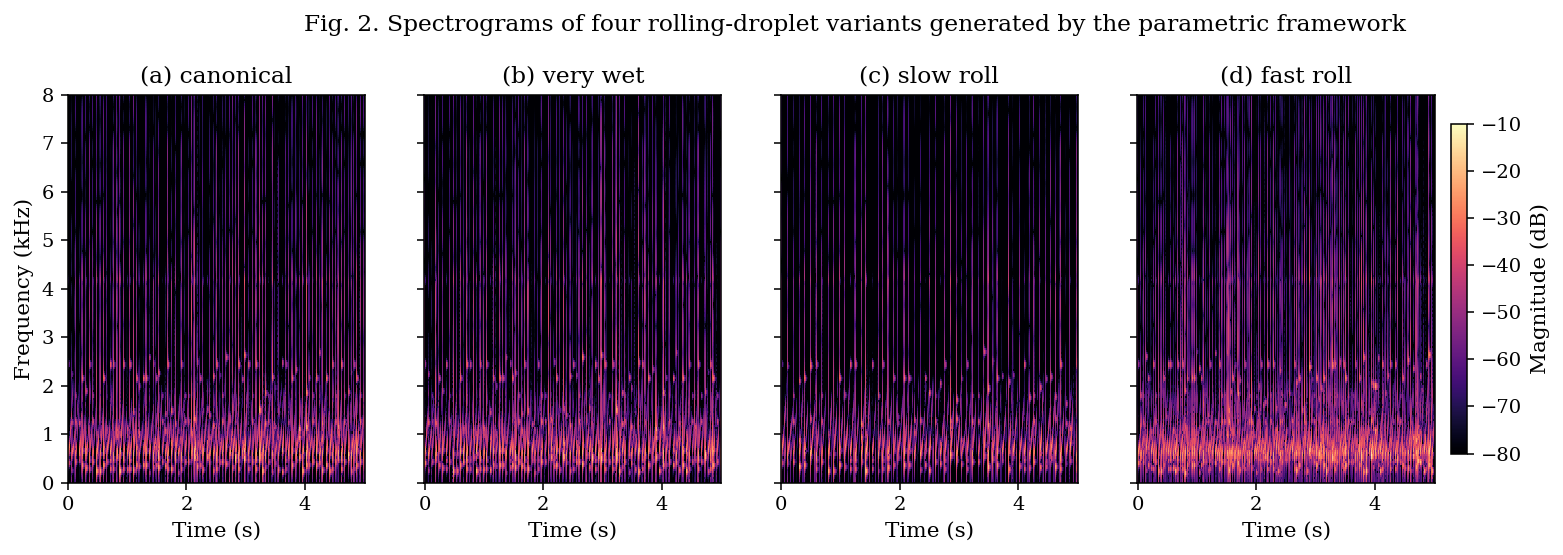
\includegraphics[width=\linewidth]{../../figures/F2_rolling_droplet_spectrograms.png}
\caption{Espectrogramas de cuatro variantes de la gota rodante generadas por el marco paramétrico.}
\label{fig:specs}
\end{figure}

% ============================================================
\section{Evaluación}
% ============================================================

\subsection{Corpus de estímulos}

Renderizamos 24 estímulos agrupados como tres escenas por ocho variantes: una gota rodante, un impacto rocoso húmedo (impacto de roca con superposición de salpicadura líquida de peso variable) y un raspado de grava mojada (grava raspando bajo superposición de vertido líquido). Todos los estímulos son de 5\,s, mono, 44,1\,kHz, normalizados a 0,95 de pico ($\approx -0{,}45$\,dBFS), y se acompañan de un registro con todos los parámetros y métricas de calidad por clip.

\subsection{Métricas objetivas}

Computamos seis métricas acústicas en cada audio: RMS y pico en dBFS, factor de cresta, planitud espectral, centroide espectral y rango dinámico. Un veredicto de calidad compuesto en \{bueno, sospechoso, defectuoso\} integra las métricas con umbrales calibrados para detectar silencios, ausencia de transitorios, ruido blanco o siseo aislado. La Tabla~\ref{tab:master} compara el marco físico con baselines neurales sobre rangos métricos idénticos.

\begin{table}[htbp]
\caption{Comparación maestra de métodos sobre generaciones de sonidos imposibles.}
\label{tab:master}
\centering\small
\begin{tabular}{lrrrrr}
\toprule
\textbf{Método} & \textbf{n} & \textbf{\% bueno} & \textbf{dyn (dB)} & \textbf{RMS (dB)} & \textbf{centroide (Hz)} \\
\midrule
\textbf{Físico (24 variantes)} & 24 & \textbf{100,0} & 36,1 & $-25{,}1$ & 3282 \\
Neural A (dirección latente) & 162 & 100,0 & 45,8 & $-28{,}6$ & 4002 \\
Neural B (edición por gradiente) & 24 & 100,0 & 59,2 & $-32{,}8$ & 2987 \\
Baseline suma aditiva & 6 & 100,0 & 11,2 & $-17{,}3$ & 451 \\
Baseline interpolación lineal & 6 & \textbf{16,7} & 38,9 & $-48{,}2$ & 3409 \\
\bottomrule
\end{tabular}
\end{table}

El marco físico, ambos baselines neurales y el baseline aditivo pasan el veredicto al 100\,\% (Tabla~\ref{tab:master}). El baseline de interpolación lineal falla en 5 de 6 casos, como anticipa el criterio de intermediación.

\subsection{Monotonía}
\label{sec:monotonia}

Para cada par (escena, parámetro) renderizamos siete estímulos barriendo el parámetro de 0 a 1 con los demás fijados en su valor central, y computamos la correlación de Spearman entre el valor del parámetro y cinco métricas acústicas: RMS, rango dinámico, centroide espectral, planitud espectral y distancia log-espectral al estímulo central. Un par es \emph{monotónico} si al menos una métrica satisface $|\rho| > 0{,}7$. De los 15 pares (tres escenas por cinco parámetros), diez son monotónicos. De los cinco restantes, cuatro corresponden a parámetros sin efecto alguno en su escena ($\rho = 0$ exacto): la resonancia en la gota rodante y en el raspado de grava (ni la gota ni los eventos granulares tienen resonancia de cuerpo ajustable), la rigidez en el raspado de grava y la granularidad en el impacto rocoso (la granularidad es un atributo de los flujos, no de impactos únicos). El quinto, la continuidad en el raspado de grava, produce variación acústica pero por debajo del umbral ($|\rho|_\mathrm{máx} = 0{,}54$). Cabe destacar la rigidez en la gota rodante: el motor la reutiliza como radio inverso de la gota (una gota más ``rígida'' se modela más pequeña), por lo que resulta fuertemente monotónica vía la relación de Minnaert ($|\rho|_\mathrm{máx} = 0{,}89$; centroide $0{,}86$). La Figura~\ref{fig:heatmap} reporta el mapa de calor de $|\rho_\mathrm{máx}|$ por par, y la Figura~\ref{fig:sweeps} muestra cinco barridos monotónicos representativos.

\begin{figure}[htbp]
\centering
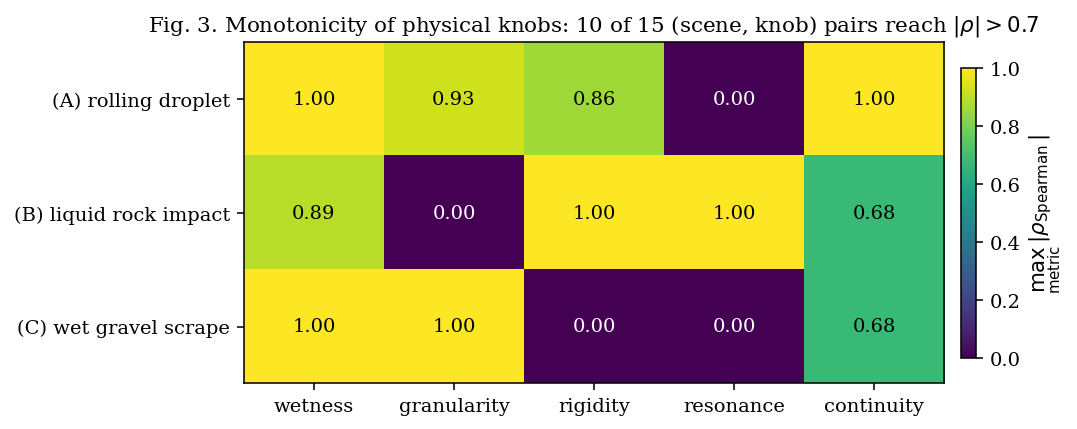
\includegraphics[width=0.9\linewidth]{../../figures/F3_monotonicity_heatmap.png}
\caption{Monotonía de los parámetros físicos: 10 de 15 pares (escena, parámetro) alcanzan $|\rho|>0{,}7$.}
\label{fig:heatmap}
\end{figure}

\begin{figure}[htbp]
\centering
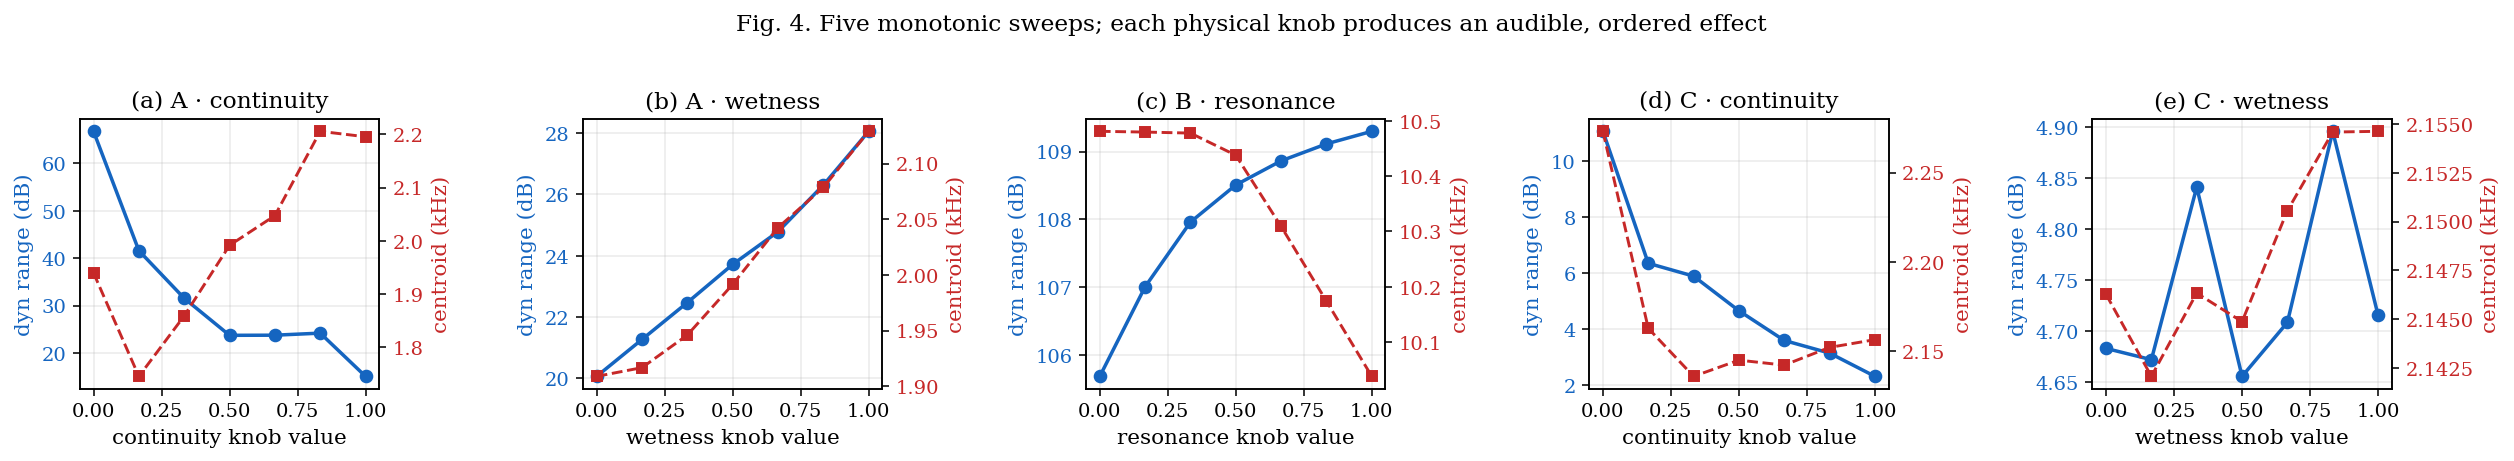
\includegraphics[width=\linewidth]{../../figures/F4_sweep_curves.png}
\caption{Cinco barridos monotónicos: cada parámetro físico produce un efecto audible y ordenado.}
\label{fig:sweeps}
\end{figure}

Crucialmente, los barridos de dirección latente neural — re-medidos sobre cuatro combinaciones disponibles de experimentos previos — son también monotónicos en métricas espectrales (4 de 4). El marco físico y los baselines neurales son, por tanto, indistinguibles en este test objetivo de monotonía. Lo que los separa es si la monotonía espectral se traduce en monotonía perceptual; esa disociación vuelve a manifestarse, medida, en la Sección~\ref{sec:fusion}, donde un índice compuesto diseñado para ordenar candidatos de fusión resulta anticorrelado con el defecto perceptual que pretende detectar.

% ============================================================
\section{Recuperación diferenciable de parámetros}
% ============================================================

Una contraparte completamente diferenciable del motor permite \emph{invertir} cualquier audio objetivo hacia los parámetros físicos del marco. Reescribimos las primitivas principales como un grafo de cómputo diferenciable, de modo que el gradiente de una pérdida espectral fluye hasta cada parámetro físico, y recuperamos dichos parámetros minimizando una pérdida de STFT multi-resolución con descenso de gradiente y una tasa de aprendizaje suficientemente lenta. Los resultados son cualitativamente distintos por primitiva, como resume la Tabla~\ref{tab:recovery}: la gota y el modal se recuperan con error inferior al 0,3\,\% cuando la inicialización es adecuada, el granular queda matemáticamente mal condicionado por la redundancia entre frecuencia base y dispersión, la reverberación recupera magnitud pero no fase, y en la fricción el decaimiento del cuerpo tiende a colapsar.

Este continuo — de recuperación quirúrgica (gota, modal) a honestamente mal condicionada (granular) — es en sí mismo un resultado: distingue qué partes del modelo físico están localmente identificables desde el audio y cuáles requieren conocimiento previo.

\textbf{El problema inverso de frecuencia.} La recuperación parcial no es un defecto de implementación sino una patología intrínseca y reconocida: la estimación de frecuencia por descenso de gradiente sobre pérdidas espectrales sufre gradientes abruptos o nulos y superficies de error pobladas de mínimos locales~\cite{hayes2022sinusoidal,uzrad2024diffmoog}; cuando las frecuencias predicha y objetivo dejan de solaparse, el gradiente de la pérdida de magnitud se anula y el optimizador se estanca. La gota rodante ocupa el extremo mal condicionado de este continuo: su radio incide sobre todo en la frecuencia del tono de Minnaert, un único rasgo espectral que compite con una rica capa modal de superficie, de modo que el mínimo de la pérdida no coincide en general con el radio verdadero; reinicios aleatorios mitigan el sesgo del radio pero no resuelven la degeneración entre viscosidad y tensión superficial. Pérdidas perceptualmente fundamentadas, como el scattering tiempo--frecuencia conjunto o la pérdida perceptual-neuronal-física~\cite{han2023pnp}, prometen gradientes más informativos.

\begin{table}[htbp]
\caption{Resumen de la recuperación inversa por primitiva.}
\label{tab:recovery}
\centering\small
\begin{tabular}{lll}
\toprule
\textbf{Primitiva} & \textbf{Error típico} & \textbf{Observación} \\
\midrule
Gota & radio $<0{,}05$\,\%, viscosidad $<0{,}2$\,\% & ninguna \\
Modal & frecuencia $<0{,}3$\,\%, decaim. $\sim1$\,\% & init de picos espectrales crítico \\
Granular & dispersión $<0{,}5$\,\%; base $\sim60$\,\% & redundancia base--dispersión \\
Reverb. & magnitud sí, fase no & pérdida insensible a la fase \\
Fricción & dureza $\sim1{,}5$\,\%, velocidad $\sim4$\,\% & decaim. del cuerpo colapsa \\
\bottomrule
\end{tabular}
\end{table}

% ============================================================
\section{Fusión de identidad: quimeras auditivas con registro alineado}
\label{sec:fusion}
% ============================================================

La quimera auditiva de Smith, Delgutte y Oxenham~\cite{smith2002chimeras} resuelve la mezcla imposible por decreto: el padre A aporta la envolvente por banda y el padre B la estructura fina, y el resultado es una única señal por construcción, no la superposición de dos. Pero la variante coloreada del compositor normaliza la envolvente de A banda a banda ($e_\mathrm{norm} = env_a / \overline{env_a}$), lo que descarta su nivel absoluto: en una banda donde A carece de energía, la normalización amplifica ruido numérico hasta amplitud unidad y esa banda emite el padre B crudo, sin modular — el percepto de dos capas~\cite{bregman1990asa} que la fusión pretendía evitar. En trueno\_hecho\_de\_agua, tres de las seis bandas del padre A quedan huérfanas así, a $-56,3$, $-85,0$ y $-94,6$\,dB relativos al pico de la banda más fuerte. El factor de cresta detecta el síntoma sin inspeccionar bandas: el baseline V11 de esa misma pareja mide 47,5\,dB de cresta a 6\,s (47,7\,dB a 8\,s), muy por encima de los 10--20\,dB de audio sano y de los 19,5\,dB que mide el mismo baseline en oceano\_hecho\_de\_campana a 6\,s (20,0\,dB a 8\,s), sin bandas huérfanas. Las dos parejas de menor solape espectral de partida — trueno\_hecho\_de\_agua (0,369) y trueno\_hecho\_de\_canica (0,084) — son, no por casualidad, las únicas con tres bandas huérfanas; ninguna otra pareja supera las dos.

Slaney, Covell y Lassiter~\cite{slaney1996morph} sostienen que fundir dos sonidos de registro distinto se percibe como dos objetos, y que alinear el registro antes de fundir colapsa la percepción en uno. En un motor paramétrico esa alineación es física exacta, no una heurística: el radio de la burbuja se despeja directamente de la relación de Minnaert, $r=3,26/f$. La Tabla~\ref{tab:sso} da el solape espectral (Bhattacharyya) sin alinear y alineando para las seis parejas del barrido. La ganancia depende de cuán disjuntos estaban los padres de partida: máxima donde no se solapaban — $4,5\times$ en trueno\_hecho\_de\_canica —, nula donde ya solapaban (canica\_hecha\_de\_fuego), y negativa en oceano\_hecho\_de\_campana, cuando el padre movido sobrepasa el objetivo. La causa no es topar con los límites del rango de alineación: de 494 candidatos con alineación activa, ninguno queda recortado. Es que padres como el vidrio y la campana invierten un modelo de fundamental única mientras la medida de registro es un centroide de banda ancha, lo que produce sobredisparos del 24\,\% al 46\,\% (fuego\_hecho\_de\_vidrio: objetivo 1193\,Hz, logrado 1743\,Hz; goteo\_hecho\_de\_campana: objetivo 691\,Hz, logrado 859\,Hz). La fricción de rodadura explica otra asimetría, visible al comparar dos objetivos de registro distintos. En canica\_hecha\_de\_fuego, mover la canica a un objetivo alto (1235\,Hz) converge con solo un 2\,\% de sobredisparo. Pero en trueno\_hecho\_de\_canica, mover la misma canica a un objetivo bajo (182\,Hz) falla al 343\,\%; sobre ese mismo objetivo bajo (182\,Hz), trueno\_hecho\_de\_agua mueve el goteo con solo un 8\,\% de sobredisparo. La canica, que modela fricción de rodadura, entrelaza esa fricción con su registro grave; el goteo, sin ese grado de libertad, ofrece un tono más limpio de ajustar.

\begin{table}[htbp]
\caption{Solape espectral (Bhattacharyya) sin alinear y alineando registro, por pareja.}
\label{tab:sso}
\centering\small
\begin{tabular}{lrr}
\toprule
\textbf{Pareja} & \textbf{sin alinear} & \textbf{alineando} \\
\midrule
trueno\_hecho\_de\_agua & 0,369 & 0,744 \\
fuego\_hecho\_de\_vidrio & 0,746 & 0,793 \\
canica\_hecha\_de\_fuego & 0,848 & 0,850 \\
trueno\_hecho\_de\_canica & 0,084 & 0,376 \\
oceano\_hecho\_de\_campana & 0,709 & \textbf{0,549} \\
goteo\_hecho\_de\_campana & 0,651 & 0,820 \\
\bottomrule
\end{tabular}
\end{table}

Construimos un índice compuesto de fusión (FCI) — coherencia de modulación, onsets huérfanos, identidad residual — para ordenar candidatos automáticamente. Sobre los 1065 candidatos con FCI definido en las seis parejas, el índice resultó anticorrelado con el objetivo: correlación de Pearson $r=+0,42$ con el factor de cresta, es decir, premia precisamente el síntoma del defecto de dos capas. Entre los candidatos de cresta sana de una misma pareja, el mejor clasificado por el FCI es la suma ponderada — el ancla de \emph{dos sonidos superpuestos} del compositor (Sección~\ref{sec:compositor}) —, no ningún candidato de fusión de identidad. Es el mismo modo de fallo que ya había invalidado un índice de unidad de stream en una iteración anterior de este trabajo. Conecta directamente con la disociación entre monotonía cuantitativa y monotonía perceptual planteada en la Introducción y medida en la Sección~\ref{sec:monotonia}, ahora en la forma \emph{una métrica de fusión no ordena lo que el oído ordena}. En su lugar filtramos por factor de cresta relativo a cada pareja y cubrimos el espacio de parámetros por barrido en vez de por ranking automático. La validación perceptual formal de este criterio de filtrado queda fuera del alcance de este trabajo.

\begin{figure}[htbp]
\centering
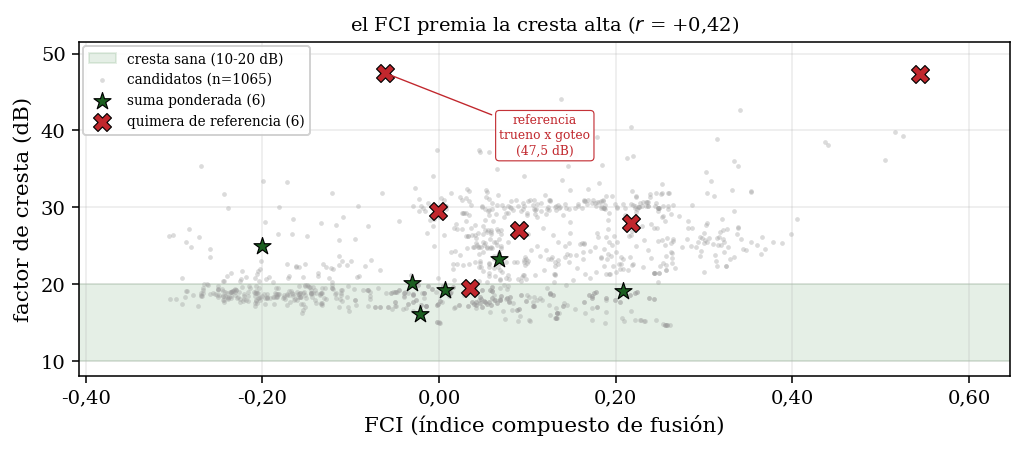
\includegraphics[width=\linewidth]{../../figures/F6_fusion.png}
\caption{Izquierda: relación entre el índice compuesto de fusión (FCI) y el factor de cresta sobre 1065 candidatos: el eje que debía penalizar el defecto de dos capas lo premia. Derecha: efecto de alinear el registro sobre el solape espectral de las seis parejas del barrido, incluida la única que empeora.}
\label{fig:fusion}
\end{figure}

% ============================================================
\section{Discusión}
% ============================================================

El marco \textbf{no aprende deliberadamente}: cada primitiva está diseñada a mano, cada modificador es función de parámetros físicos, y la cadena entera es determinista. Los beneficios son reproducibilidad, interpretabilidad y ausencia de requisitos de datos de entrenamiento; los costes son el alcance, ya que cada material e interacción requiere una decisión de modelado, y la imposibilidad de generalizar a combinaciones realmente nuevas sin intervención humana. Vemos el marco como el \emph{profesor} en un futuro escenario profesor--alumno: un modelo neural entrenado para invertir parámetros físicos desde grabaciones reales, con el motor físico generando supervisión bajo demanda.

Los baselines neurales con dirección latente destacan un confundente recurrente en la literatura: la monotonía espectral es necesaria pero no suficiente para el control perceptual. Un método que cambia el RMS y el centroide de forma monotónica puede aún producir audio que los oyentes no ordenan a lo largo del eje semántico pretendido. El marco físico colapsa esa brecha por construcción; la cuestión abierta es si los oyentes coinciden.

\textbf{Limitaciones.} El marco está restringido a los materiales e interacciones tabulados. Los perfiles modales están afinados a mano y se beneficiarían de calibración data-driven contra respuestas al impulso reales. El modelo de líquido emplea la burbuja de Minnaert como aproximación de primer orden; estrictamente, esta resonancia describe la burbuja entrañada en el agua receptora en el instante del contacto, no una burbuja contenida en la gota en vuelo, e ignora el acoplamiento entre burbujas y los desplazamientos de frecuencia por forma e interfaz que caracterizan el estado del arte en acústica de fluidos~\cite{xue2023coupled,langlois2016bubbles}; incorporar modos acoplados es una vía natural de mejora. Finalmente, la gota rodante, aunque audiblemente reconocible, es una realización de una clase: distintas superficies y formas de gota requerirían validación de parámetros aún pendiente.

% ============================================================
\section{Conclusiones}
% ============================================================

Hemos presentado un marco paramétrico físicamente informado para sintetizar sonidos imposibles, con la gota rodante como caso paradigmático. El marco soporta combinaciones imposibles materia--interacción mediante primitivas en capas y un compositor genérico. Las métricas acústicas confirman control monotónico donde es físicamente aplicable, y la fusión de identidad extiende la misma disociación entre monotonía cuantitativa y perceptual a las combinaciones de material: alinear el registro mejora el solape espectral de partida salvo cuando el padre movido sobrepasa el objetivo, y un índice compuesto pensado para ordenar candidatos automáticamente resulta anticorrelado con el defecto que debía detectar; la validación perceptual formal de ambos resultados queda fuera del alcance de este trabajo. Una contraparte diferenciable cierra el bucle inverso, recuperando parámetros físicos desde audio con un continuo de identificabilidad que el trabajo documenta explícitamente, desde la recuperación quirúrgica de gotas e impactos modales hasta casos mal condicionados como la propia gota rodante, cuyo cuello de botella es la estimación de frecuencia por gradiente. Situado frente al estado del arte reciente, el marco es una demostración interpretable y reproducible de modelado físico diferenciable cuya principal vía de mejora es la adopción de física de burbujas acopladas. El código, el conjunto de datos y la demostración interactiva se liberan de forma anónima para revisión y públicamente tras la aceptación.

% ============================================================
\section*{Reproducibilidad}
% ============================================================

Todo el audio del artículo se genera con código determinista, con tiempos de CPU separados por etapa: los estímulos, las tablas de monotonía y las figuras se generan en pocos minutos; el barrido de fusión de la Sección~\ref{sec:fusion} — 1065 candidatos sobre seis parejas — toma del orden de una hora medida en CPU, paralelizable por pareja. El conjunto de demostración se genera aparte. Cada ajuste inverso persiste sus parámetros recuperados, errores y trayectoria de pérdida como informe JSON, de modo que las cifras de la Tabla~\ref{tab:recovery} son trazables a artefactos versionados; las cifras de la Sección~\ref{sec:fusion} lo son igualmente a los CSV versionados en \texttt{results/fusion\_search/}. Se acompaña además una demostración interactiva en navegador, con las primitivas portadas a una página autónoma desplegable en cualquier alojamiento estático. Código, datos y demostración se publican junto al artículo.

% ============================================================
\begin{thebibliography}{99}
\footnotesize

\bibitem{defossez2022encodec}
A.~D{\'e}fossez \emph{et al.},
``High fidelity neural audio compression,''
\emph{arXiv:2210.13438}, 2022.

\bibitem{caillon2021rave}
A.~Caillon and P.~Esling,
``RAVE: A variational autoencoder for fast and high-quality neural audio synthesis,''
\emph{arXiv:2111.05011}, 2021.

\bibitem{kumar2023dac}
R.~Kumar \emph{et al.},
``High-fidelity audio compression with improved RVQGAN,''
\emph{NeurIPS}, 2023.

\bibitem{liu2023audioldm}
H.~Liu \emph{et al.},
``AudioLDM: Text-to-audio generation with latent diffusion models,''
\emph{ICML}, 2023.

\bibitem{evans2024stableaudio}
Z.~Evans \emph{et al.},
``Stable Audio Open,''
\emph{Stability AI Technical Report}, 2024.

\bibitem{roche2021autoencoders}
F.~Roche \emph{et al.},
``Autoencoders for music sound modeling: A comparison of linear, shallow, deep, recurrent and variational models,''
\emph{Frontiers in Signal Processing}, 2021.

\bibitem{devis2023control}
N.~Devis \emph{et al.},
``Continuous descriptor-based control for deep audio synthesis,''
\emph{ICASSP}, 2023.

\bibitem{minnaert1933}
M.~Minnaert,
``On musical air-bubbles and the sounds of running water,''
\emph{The London, Edinburgh, and Dublin Philosophical Magazine}, vol.~16, no.~104, 1933.

\bibitem{vandendoel2005physically}
K.~van~den~Doel,
``Physically based models for liquid sounds,''
\emph{ACM Transactions on Applied Perception}, vol.~2, no.~4, 2005.

\bibitem{drumm2010bubble}
I.~Drumm,
``Synthesis of bubble sounds,''
\emph{Internoise}, 2010.

\bibitem{xue2023coupled}
K.~Xue, J.~Aronson, D.~Wang, T.~Langlois, and D.~L.~James,
``Improved water sound synthesis using coupled bubbles,''
\emph{ACM Transactions on Graphics (SIGGRAPH)}, vol.~42, no.~4, 2023.

\bibitem{langlois2016bubbles}
T.~R.~Langlois, C.~Zheng, and D.~L.~James,
``Toward animating water with complex acoustic bubbles,''
\emph{ACM Transactions on Graphics (SIGGRAPH)}, vol.~35, no.~4, 2016.

\bibitem{bilbao2009numerical}
S.~Bilbao,
\emph{Numerical Sound Synthesis: Finite Difference Schemes and Simulation in Musical Acoustics}.
Wiley, 2009.

\bibitem{avanzini2006friction}
F.~Avanzini and S.~Crosato,
``Friction models for sound synthesis,''
\emph{Proc.\ DAFx}, 2006.

\bibitem{barahona2024noisebandnet}
A.~Barahona-R{\'i}os and T.~Collins,
``NoiseBandNet: Controllable time-varying neural synthesis of inharmonic sounds,''
\emph{IEEE Trans.\ Audio, Speech, Lang.\ Process.}, 2024.

\bibitem{lee2023learning}
B.~Lee \emph{et al.},
``Learning control of neural sound effects synthesis from physically inspired models,''
\emph{Proc.\ AES}, 2023.

\bibitem{soundmorpher2023}
[SoundMorpher],
``SoundMorpher: A unified framework for sound morphing,''
\emph{Proc.\ DAFx}, 2023.

\bibitem{wu2023clap}
Y.~Wu \emph{et al.},
``Large-scale contrastive language-audio pretraining (CLAP),''
\emph{ICASSP}, 2023.

\bibitem{engel2020ddsp}
J.~Engel \emph{et al.},
``DDSP: Differentiable digital signal processing,''
\emph{ICLR}, 2020.

\bibitem{jin2024diffsound}
X.~Jin \emph{et al.},
``DiffSound: Differentiable modal sound rendering and inverse rendering for diverse inference tasks,''
\emph{ACM SIGGRAPH}, 2024.

\bibitem{lee2024modal}
J.~W.~Lee \emph{et al.},
``Differentiable modal synthesis for physical modeling of planar string sound and motion simulation,''
\emph{NeurIPS}, 2024.

\bibitem{hayes2022sinusoidal}
B.~Hayes, C.~Saitis, and G.~Fazekas,
``Sinusoidal frequency estimation by gradient descent,''
\emph{arXiv:2210.14476}, 2022.

\bibitem{uzrad2024diffmoog}
N.~Uzrad \emph{et al.},
``DiffMoog: A differentiable modular synthesizer for sound matching,''
\emph{arXiv:2401.12570}, 2024.

\bibitem{han2023pnp}
H.~Han, V.~Lostanlen, and M.~Lagrange,
``Perceptual-neural-physical sound matching,''
\emph{ICASSP}, 2023.

\bibitem{smith2002chimeras}
Z.~M.~Smith, B.~Delgutte, and A.~J.~Oxenham,
``Chimaeric sounds reveal dichotomies in auditory perception,''
\emph{Nature}, vol.~416, no.~6876, pp.~87--90, 2002.

\bibitem{slaney1996morph}
M.~Slaney, M.~Covell, and B.~Lassiter,
``Automatic audio morphing,''
\emph{Proc.\ IEEE ICASSP}, pp.~1001--1004, 1996.

\bibitem{mcdermott2011texture}
J.~H.~McDermott and E.~P.~Simoncelli,
``Sound texture perception via statistics of the auditory periphery: Evidence from sound synthesis,''
\emph{Neuron}, vol.~71, no.~5, pp.~926--940, 2011.

\bibitem{bregman1990asa}
A.~S.~Bregman,
\emph{Auditory Scene Analysis: The Perceptual Organization of Sound}.
MIT Press, 1990.

\end{thebibliography}

\end{document}
